%template1.tex
%The following LaTeX source file represents the simplest kind of slide presentation; no overlays, no included graphics. Substitute your favorite style for ``pascal''. To create the PDF file template1.pdf, (1) be sure to use the prosper class, then (2) execute the command latex template1.tex, and (3) the command dvipdf template1.dvi.

%%%%%%%%%%%%%%%%%%%%%%%%%%%%%%% template1.tex %%%%%%%%%%%%%%%%%%%%%%%%%%%%%%%%%%%
\documentclass[a4paper,blends,pdf,colorBG,slideColor]{prosper}
% definitions for slides for CSC544
% Lutz Hamel, (c) 2007

\hypersetup{pdfpagemode=FullScreen}

\usepackage{times}
\usepackage{latexsym}
\usepackage{alltt}
\usepackage{booktabs}
\usepackage{amsmath}
\usepackage{amsopn}
\usepackage{amsfonts}
\usepackage{amssymb}
%\usepackage[usenames]{color}

\def\sign{\qopname\relax{no}{sign}}
\def\argmax{\qopname\relax{no}{argmax}}
\def\argmin{\qopname\relax{no}{argmin}}

\newcommand{\grad}{\ensuremath{\nabla}} 
\newcommand{\loss}{\ensuremath{{\cal L}}}
\newcommand{\err}{\mbox{err}}
\newcommand{\mse}{\mbox{mse}}
\newcommand{\acc}{\mbox{acc}}
\newcommand{\Integer}{\ensuremath{\mathbb{N}}}
\newcommand{\size}[1]{{|{#1}|}}
\newcommand{\Rnspace}[1]{\ensuremath{\mathbb{R}^{#1}}}
\newcommand{\Real}{\ensuremath{\mathbb{R}}}
\newcommand{\mytt}[1]{{\small\tt{#1}}}
\newcommand{\textemph}[1]{{\em #1}}
\newcommand{\suchthat}{\mid}
\newcommand{\orbar}{\;|\;}
\newcommand{\bs}[1]{\begin{slide}{#1}\ptsize{8}}
\newcommand{\es}{\end{slide}}
\newcommand{\co}{\,\colon\;}
\newcommand{\pair}[2]{\ensuremath{( {#1}, {#2} )}}
\newcommand{\model}[1]{\hat{#1}}
\newcommand{\ul}[1]{{\bf\em #1}}
\newcommand{\ol}{\overline}
\newcommand{\definition}[1]{{\bf Definition: }{\em #1}}
\newcommand{\example}[1]{{\bf Example: }{#1}}
\newcommand{\abs}[1]{|{#1}|}
\newcommand{\mytab}{\makebox[.1in]{}}

\newcommand{\fdef}[1]{
\begin{center}
\fbox{
\begin{minipage}{3.5in}
{\bf Definition:}
{#1}
\end{minipage}
}
\end{center}
}

\newcommand{\fframe}[1]{
\begin{center}
\fbox{
\begin{minipage}{3.5in}
{#1}
\end{minipage}
}
\end{center}
}

\newcommand{\nframe}[1]{
\begin{center}
\begin{minipage}{3.5in}
{#1}
\end{minipage}
\end{center}
}

\newenvironment{Rcode}
	{
		\scriptsize
		\begin{quote}
		\begin{alltt}
	}
	{
		\end{alltt}
		\end{quote}
	}




\begin{document}

\bs{Learning \& Decision Surfaces}
The techniques from linear algebra developed so far allow us to precisely describe decision
surfaces for binary classification problems.

{\bf Definition:} {\bf\em Decision surfaces} are (hyper)planes that separate points in a dot product space
according to their classification label.
\es

\bs{Decision Surfaces \& Functions}

Let us cast our classification problem into the machine learning framework:
\begin{itemize}
\item Let some dot product space $\Rnspace{n}$ be our data universe with points $\ol{x} \in \Rnspace{n}$.
\item Let $S$ be a sample set such that $S \subset \Rnspace{n}$.
\item Let $f\co \Rnspace{n} \rightarrow \{-1,+1\}$ be the target function
\item Let $D = \{\langle \ol{x}, f(\ol{x})\rangle \mid \ol{x} \in S\}$
be the training set.
\end{itemize}
Compute a function $\model{f}\co \Rnspace{n} \rightarrow \{+1,-1\}$ using $D$ such that
\[
\model{f}(\ol{x}) \cong f(\ol{x}) \mbox{ for all } \ol{x} \in \Rnspace{n}.
\]
Let us assume that our training set is $D = \{\pair{\ol{x}_1}{y_1},\pair{\ol{x}_2}{y_2},\ldots,\pair{\ol{x}_n}{y_n}\}$ with $y_i \in \{+1, -1\}$, is linearly separable. That is, we assume that 
 we are guaranteed to find a hyperplane that
separates the two classes.
We also assume that we can compute a hyperplane that goes through the origin, 
\[
g(\ol{x}) = \ol{w}\bullet\ol{x}=0
\]
and separates the two classes.  We call $g$ a {\bf\em decision surface}.
\es

\bs{Decision Surfaces \& Functions}
If we assume that our dot product space is the two dimensional real space $\Rnspace{2}$,
then we can represent a decision surface $g(\ol{x})$ as a line  that goes through the origin (a):

\begin{center}
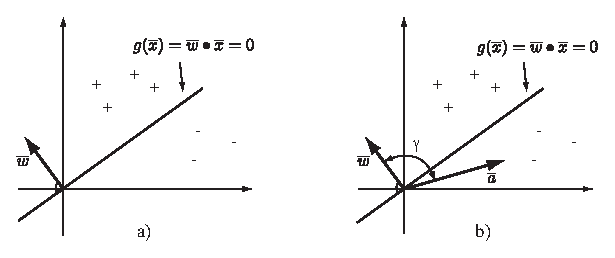
\includegraphics[height=30mm]{figures/fig04-01.eps}
\end{center}

In (b) notice that our decision surface $g(\ol{x})$ will produce 
positive values for points that lie above the surface ($\gamma < 90^\circ$) 
 and negative values for points that lie below it ($\gamma > 90^\circ$).  
\es

\bs{Decision Surfaces \& Functions}
Instead of
scalar positive and negative values we want our model $\model{f}$ to compute the labels
$+1$ and $-1$, so we use the decision surface $g(\ol{x})$ to construct our model as follows,
\[
\model{f}(\ol{x}) = \left\{
\begin{array}{ll}
+1 & \mbox{if $g(\ol{x}) \ge 0$}\\
-1 & \mbox{otherwise}
\end{array}
\right.
\]
Our model $\model{f}$ is also called a {\bf\em decision function}.

\es

\bs{Decision Surfaces \& Functions}
Let us relax the requirement that our decision surface needs to go through the origin.  What would
our decision function look like in this case?

We can derive it as follows.  Consider the following graphs.
\begin{center}
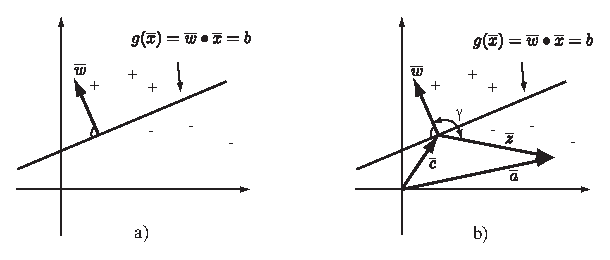
\includegraphics[height=35mm]{figures/fig04-02.eps}
\end{center}
Part (a) shows a decision function $g(\ol{x}) = \ol{w}\bullet\ol{x} = b$ with the offset term $b$.
Part (b) shows that we can no longer simply take the angle between the position vector of the point we
want to classify $\ol{a}$ and the normal vector $\ol{w}$.
\es

\bs{Decision Surfaces \& Functions}
The trick here is to pick a point $\ol{c} \in g$ or
\begin{equation*}
g(\ol{c}) = \ol{w}\bullet\ol{c} = b,
\end{equation*}
that can act as our origin for classification purposes.
Then we can pick a $\ol{z}$ such that $\ol{a} = \ol{c} + \ol{z}$ or
\begin{equation*}
\ol{z} = \ol{a} - \ol{c}.
\end{equation*}
Observe that
\begin{equation*}
\ol{w}\bullet\ol{z} = \abs{\ol{w}}\abs{\ol{z}}\cos \gamma
\end{equation*}
will give us the correct classification of point $\ol{a}$.  Formally,
\begin{align*}
\ol{w}\bullet\ol{z} &= \ol{w}\bullet(\ol{a} - \ol{c}) \\
	&= \ol{w}\bullet\ol{a} - \ol{w}\bullet\ol{c} \\
	&= \ol{w}\bullet\ol{a} -b \\
	&= g(\ol{a}) - b
\end{align*}
This means that we can compute the classification value of some point $\ol{a}$ by first
applying the decision surface and then subtracting the offset term.
\es

\bs{Decision Surfaces \& Functions}
We can now construct our decision function as
 \begin{equation*}
\model{f}(\ol{x}) = \left\{
\begin{array}{ll}
+1 & \mbox{if $g(\ol{x}) -b \ge 0$,}\\
-1 & \mbox{if $g(\ol{x})-b < 0$,}
\end{array}
\right.
\end{equation*}
for all $\ol{x}\in \Rnspace{2}$.

Note that decision functions based on decision surfaces that run through the origin are simply
a special case of the decision function above with $b=0$.

Also note that this construction easily generalizes to arbitrarily dimensioned real spaces $\Rnspace{n}$
since none of the construction depends on the dimensionality of the underlying space.
\es

\end{document}
%%%%%%%%%%%%%%%%%%%%%%%%%%% end of template1.tex %%%%%%%%%%%%%%%%%%%%%%%%%%%%%%%%

